\section{Internals}
\subsection{Problem Set up and Formulation}

The basic causal model in statistics is called the
\ignore{Neyman-Rubin Causal Model (NRCM) (also referred to as}
{\em potential outcome framework (POF)}.
In this model, we are given a table with $N$ rows called {\em units} indexed by $i=1 \ldots N$ (see
Table~ \ref{fig:causal:inference}).  The binary attribute $T$ denotes {\em treatment assignment}.
%sr: already in first para. ($T=1$ means the unit was treated; $T=0$ means the unit was subjected to control);
$X$ is a vector of
background characteristics, (e.g., sex, race, age, \ldots) of each unit,
called {\em covariates}, unaffected by treatment; and the two
attributes $Y(0), Y(1)$ represent {\em potential outcomes}: $Y(1)$ is
the outcome of the unit if it is exposed to the treatment and $Y(0)$
is the outcome when it is exposed to the control.

%For any attribute $T$, we write $T_i$ for the value of the $i$'s unit.
The {\em treatment effect}
caused by the treatment $T_i$ for the $i$th unit  is defined as $Y_i(1)-Y_i(0)$.
The goal of causal analysis is to compute the {\em average treatment
  effect (ATE)}:   ATE = E[Y(1)-Y(0)] = E[Y(1)] - E[Y(0)].
\begin{figure}
  \centering
{\scriptsize
  \begin{tabular}{|c|c|c|c|c|c|} \hline
    Unit & Covariates & Treatment & Treatment & Control & Causal  Effect \\
   & $X$ & assignment $T$ & outcome $Y(1)$ & outcome $Y(0)$ & $Y(1)-Y(0)$ \\
    \hline
    1 & $X_1$ & $T_1$ & $Y_1(1)$ & $Y_1(0)$ & $Y_1(1) - Y_1(0)$ \\
    2 & $X_2$ & $T_2$ & $Y_2(1)$ & $Y_2(0)$ & $Y_2(1) - Y_2(0)$ \\
    $\ldots$ & $\ldots$ & $\ldots$ & $\ldots$ & $\ldots$ & $\ldots$ \\
    N & $X_N$ & $T_N$ & $Y_N(1)$ & $Y_N(0)$ & $Y_N(1) - Y_N(0)$ \\ \hline
  \end{tabular}
}
\caption{The Potential Outcome Framework~\cite{Rubin2005}}
  \label{fig:causal:inference}
  \vspace{-3mm}
\end{figure}
\noindent
The so-called {\em fundamental problem of causal inference (FPCI)} is that
for each unit we only know either $Y(1)$ or $Y(0)$ but not both. Thus, further assumption is needed for estimating ATE. \ignore{
\cite{Holland1986}, and causal inference is reduced to a missing data
problem \cite{RosenbaumRubin1983}. }


The strongest is the {\em independence assumption}, which states that
the treatment mechanism is independent of the potential outcomes,
i.e., $(Y(1), Y(0)) \bigCI T$. Then, it holds that
$\E[Y(1)]=\E[Y(1)|T=1]$ and similarly $\E[Y(0)]=\E[Y(0)|T=0]$ and we
have:  ATE = E[Y(1)|T=1]-E[Y(0)|T=0]. \label{eq:indeass}

In observational data, the mechanism used to assign treatments
to units is not known, thus independence fails in general.  For
example, thunder occurs mostly in the summer, which is also high
travel season, and therefore delays may be caused by the high traffic.
In that case $T$ and $Y(0)$ (the delay when thunder does not occur)
are correlated, since they are high in the summer and low in the
winter, and similarly for $T$ and $Y(1)$.  \ignore{The vast majority of datasets
available to analysts today are observational data, and this motivates
our interest in this case.}  Here, statistical literature makes the
following weaker assumption~\cite{Rubin1983b} called {\em Strong Ignorability}: Forall $x$ the following hold:
  (1) Unconfoundedness $({Y(0), Y(1) \bigCI T} | X=x)$ and
  (2) Overlap $0 < \textrm{Pr}(T = 1 | X=x) < 1$.



\ignore{
The first part, {\em unconfoundedness}, means that, if we partition
the data by the values of the covariate attributes $X=x$, then, within
each group, the treatment assignment and the potential outcomes are independent; then we can
estimate $\ate$ by computing Eq. \ref{eq:indeass} for each value of
the covariates $X=x$ (i.e., conditioning on $X$) and averaging.  The
second part, {\em overlap} is needed to ensure that the conditional
expectations $\E[Y(1)|T=1,X=x]$ and $\E[Y(0)|T=0,X=x]$ are well
defined.  However, once we include sufficiently many covariate attributes $X$
(as we should) then the data becomes sparse, and many groups $X=x$ are
either empty or have a very small number of items.  For example if a
group has only treated units, then the overlap condition fails, in
other words the conditional expectation $\E[Y(0)|X=x,T=0]$ is
undefined.}

\ignore{
\begin{eqnarray}
% \nonumber % Remove numbering (before each equation)
  ATE &=& E_x[E[Y(1)-Y(0)| X=x]] \nonumber \\
   &=& E_x[E[Y(1)|T=1,X=x]]  -E_x[E[Y(0)|T=0, X=x]] \nonumber \\ \label{eq:oatt}
\end{eqnarray}}

\ignore{
ATE ~~=~~ E_x[E[Y(1)-Y(0)| X=x]] ~~ =~~ E_x[E[Y(1)|T=1,X=x]]  -E_x[E[Y(0)|T=0, X=x]]\label{eq:oatt}
\end{equation}
 }

 \ignore{
 Causal inference in the lack of randomization is called observational studies. By contrary  to the popular
belief that it is nearly impossible to infer causality from data, such inference is possible under some strict
assumptions and following the careful methodology that has been developed within the statistics, economics and social sciences literature. In this direction one of the most popular method developed for causal inference is matching. Next we overview the matching methods supported by \GSQL\ and their implementation.}

\begin{figure*} \scriptsize
  \centering
  \begin{tabular}{|l|l|l|} \hline
    \bf{Name} &  $\delta(x_i,x_j)=$ & \bf{Comments} \\ \hline
Coarsened distance & 0 if $C(x_i)=C(x_j)$ & Where $C(x)$ is a function that coarsen \\
               & $\infty$ if $C(x_i) \neq C(x_j)$ & a vector of continues covariate~\cite{IacKinPor09}\\ \hline
Propensity score  & $|E(x_i) - E(x_j)|$ & where $E(x) = \textrm{Pr}(T = 1 | X=x)$\\
distance (PS)   &  & is the propensity score~\cite{Rubin1983b} \\ \hline
Mahalanobis Distance (MD) & $(x_i-x_j)'\Sigma^{-1} (x_i-x_j)$ & where $\Sigma=$ covariance matrix~\cite{Stuart10} \\ \hline
  \end{tabular}
  \caption{Distance Measures used in Matching}
  \label{fig:metrics}
\end{figure*}

 If strong ignorability holds, one can estimate ATE by
 taking the aggregate average difference for each group i.e., $E_x[E[Y(1)-Y(0)| X=x]]$.
In practice, however, a direct application of this method is
impossible, because the data is typically very sparse: for any value
$X=x$ we either have no data values at all, or very few such values,
which means that estimating $E[Y(T)|T=1\mbox{ or }0,X=x]$ as an
average from the database leads to large sampling error. A solution adopted in statistics is {\em matching and subclassification}~\cite{Rubin1983b}.  The idea is to match each treated unit with one or multiple control
units with ``close'' values of the covariate attributes $X$, where
closeness is defined using some distance function between the covariate values of two units.  The most
commonly used distance functions are presented  in Table \ref{fig:metrics}. \ignore{The efficacy
of a matching method is evaluated by measuring {\em degree of
  imbalance} i.e., the differences between the distribution of
covariates in two groups in the matched subset. Since there is no
generic metric to compare two distributions, measures such as mean,
skewness, quantile and multivariate histogram are used for this
purpose.  \ignore{A rule of thumb is to
evaluate different distance metrics and matching methods until a
well-balance matched subset with a reasonable size obtained.}}






\subsection{Subclassification and matching algorithms}
\label{sec:algo}
This demonstration walks through the state-of-the-art matching and subclassification methods in statistics.
We also present the basic SQL statement that captures these methods. In addition, we outline the techniques
employed by \GSQL\ to perform them efficiently. In particular we demonstrate the following methods:

{\bf Nearest Neighbor Matching}
\label{sec:nnm}
The most common matching method is that of $k:1$ nearest neighbor
matching (NNM). NNM controls matches for each treated
unit and can be done with or without replacement. We denote
them respectively by NNMWR and NNMNR. In practice, matching is usually
performed without replacement.  Notice that NNM faces the risk of bad
matches if the closest neighbor is far away. This issue can be
resolved by imposing a tolerance level on the maximum distance, known
as the {\em caliper} (see e.g., \cite{lunt2014selecting}). \ignore{There are some rules of thumb for choosing the
calipers (see e.g., \cite{lunt2014selecting}).} The basic SQL statement to perform NNM is depicted in Figure \ref{fig:nnmnr}. However, \GSQL\  uses a more efficient query for this task by leveraging recent developments in the context of spatial-databases
(see \cite{obe2015postgis}).

\begin{figure}
  \centering
\begin{alltt} \scriptsize
CREATE VIEW \(\nnmnr\)
AS WITH potential_matches AS
  (SELECT treated.ID AS tID, control.ID AS cID,
          \(\delta(treated.\cv,control.\cv)\)  AS distance
   FROM \(\rel\) AS control, \(\rel\) AS treated
   WHERE control.T=0 AND treated.T=1
     AND \(\delta(treated.\cv,control.\cv)\) < \(caliper\))),
            ordered_potential_matches AS
  (SELECT *, ROW_NUMBER() over (ORDER BY distance) AS order
   FROM potential_matches)
SELECT *
FROM ordered_potential_matches AS rp
WHERE NOT EXISTS
    (SELECT *
     FROM ordered_potential_matches AS z
     WHERE z.order < rp.order AND z.cID=rp.cID)
  AND (SELECT count(*)
     FROM ordered_potential_matches AS rp
     WHERE z.order < rp.order AND z.tID=rp.tID)\( \leq k\);
\end{alltt} \vspace{-.3cm}
  \caption{\bf SQL implementation of NNMNR}\label{fig:nnmnr}
\end{figure}


\ignore{
{\bf NNM With Replacement}
We propose two alternative ways for computing  NNMWR in SQL, shown in
Figure \ref{fig:nnmwr}. In Figure \ref{fig:nnmwr}(a), each treated unit is joined with $k$ closest control units that are closer than the caliper. In this solution, nearest control units are identified by means of an anti-join. \ignore{Note that when $k=1$ the aggregate expression may be replaced by NOT EXISTS.}  In Figure \ref{fig:nnmwr}(b), all potential matches and their distances are identified by
joining the treated with the control units that are closer than
the caliper. Then, this set is sorted into ascending order of
distances.  In addition, the order of each row in the sorted set is identified
using the window function {\verb|ROW_NUMBER|}. Finally, all units with the order of less than or equal to $k$ are selected as the matched units.


The ani-join based statement requires a three-way join. \ignore{However, in a particular case when
  $k=1$ and the caliper is zero, this solution can becomes linear for
  matching based on propensity score.} The window function based
solution has a quadratic complexity. It requires a nested-loop to
perform a spatial-join and a window aggregate to impose
minimality. Note that window functions are typically implemented in
DBMS using a sort algorithm, and even more efficient algorithms have
been recently proposed~\cite{Neumann15}.






\begin{figure}
  \centering
\begin{alltt} \scriptsize
CREATE VIEW \(\nnmnr\)
AS WITH potential_matches AS
  (SELECT treated.ID AS tID, control.ID AS cID,
          \(\delta(treated.\cv,control.\cv)\)  AS distance
   FROM \(\rel\) AS control, \(\rel\) AS treated
   WHERE control.T=0 AND treated.T=1
     AND \(\delta(treated.\cv,control.\cv)\) < \(caliper\))),
            ordered_potential_matches AS
  (SELECT *, ROW_NUMBER() over (ORDER BY distance) AS order
   FROM potential_matches)
SELECT *
FROM ordered_potential_matches AS rp
WHERE NOT EXISTS
    (SELECT *
     FROM ordered_potential_matches AS z
     WHERE z.order < rp.order AND z.cID=rp.cID)
  AND (SELECT count(*)
     FROM ordered_potential_matches AS rp
     WHERE z.order < rp.order AND z.tID=rp.tID)\( \leq k\);
\end{alltt} \vspace{-.5cm}
  \caption{\bf SQL implementation of NNMNR}\label{fig:nnmnr}
\end{figure}


{\bf NNM Without Replacement} \ignore{Expressing NNMNR in a declarative manner
can be complicated. In fact,} This method aims
to minimize the average absolute distance between matched units and can performed in either greedy or optimal manner. The latter is called {\em optimal matching}
\cite{Rosenbaum93}. Before we describe our proposed SQL implementation for NNMWR, we prove
that optimal matching is not expressible in SQL: this justifies
focusing on approximate matches.  For our inexpressibility result,
notice that in the special case when $k=1$ NNMWR is the {\em weighted
  bipartite graph matching problem (WBGM)}, which is defined as
follows: given a bipartite graph $G=(V,E)$ and a weight function
$w: E \rightarrow \mathbb{R}_{>0}$, find a set of vertex-disjoint
edges $M \subseteq E$ such that $M$ minimise the total weight
$w(M) = \sum_{e \in M} w(e)$.  The exact complexity of this problem
is unknown (see, e.g. \cite{Avis83}), however we prove a \NLOGSPACE\
lower bound:

\vspace{-.2cm}
\begin{proposition} \label{pro:om}
Computing  maximum weight matching for  weighted bipartite graphs is hard for \NLOGSPACE.
\end{proposition}

\begin{proof} The following {\em Graph Reachability Problem} is known
  to be \NLOGSPACE\ complete: given a directed graph $G(V,E)$ and two
  nodes $s,t$, check if there exists a path from $s$ to $t$.  We prove
  a reduction from graph reachability to the {\em bipartite perfect
    matching problem} which is a special case of optimal WBGM. For
  that we construct the graph $G'$ with $V= V \cup V'$ where, $V'$ is
  a copy of $V$ with primed labels and
  $E'= \{(x,x')| \forall x \in V -\{s,t\} \} \cup \{(x,y')| \forall
  (x,y) \in E\} \cup \{(t,s')\}$.
  Notice that the subset $\setof{(x,x')}{x \in V} \subseteq E$ is
  almost a perfect matching, except that it misses the nodes $s, t'$.
  We prove: there exists a path from $s$ to $t$ in $G$ iff $G'$ has a
  perfect matching.  First assume $P=s, x_1, x_2, \ldots, x_m, t$ is a
  path in $G$. Then the following forms a perfect matching in $G'$:
  $M=\set{(s,x_1'), (x_1,x_2'), \ldots, (x_{m},t'), (t,s')} \cup
  \setof{(y,y')}{y \not\in \set{s,x_1, \ldots, x_m,t}}$.
  Conversely, assume $G'$ has a perfect matching. Write
  $f : V \rightarrow V'$ the corresponding bijection, i.e. every $x$
  is matched to $y'=f(x)$.  Denoting the nodes in $V$ as
  $V=\set{x_1, \ldots, x_n}$, we construct inductively the following
  sequence: $x_{i_1}' = f(s)$, $x_{i_2}' = f(x_{i_3})$, \ldots,
  $x_{i_{k+1}}' = f(x_{i_k})$.  Then $i_1, i_2, \ldots$ are distinct
  (since $f$ is a matching), hence this sequence must eventually reach
  $t'$: $t' = f(x_{i_m})$.  Then
  $s,x_{i_1},x_{i_2}, \ldots, x_{i_m}, t$ forms a path from $s$ to $t$
  in $G$.  This completes the proof.
\end{proof}

The proposition implies that optimal matching is not expressible in
SQL without the use of recursion.  Optimal matching can be solved in
\PTIME using, for example, the {\em Hungarian} algorithm, which, in
theory, could be expressed using recursion in SQL.  However, optimal
matching is rarely used in practice and, in fact, it is known that it
does not in general perform any better than the greedy NNM (discussed
next) in terms of reducing degree of covariate imbalance
\cite{Rosenbaum93}.   For that reason, we did not implement optimal
matching in our system.


1:1 NNMWR can be approximated with a simple greedy algorithm that
sorts all edges of the underlying graph in ascending order of weights
and iterates through this sorted list, marking edges as ``matched"
while maintaining the one-to-one invariant. \ignore{This algorithm can return
a maximal matching that is at least $\frac{1}{2}$-optimal
\cite{Avis83}.} Figure \ref{fig:nnmnr} adopts this greedy algorithm to
express $1:k$ NNMWR in SQL.  This algorithm is very similar to that of
NNMWR in Figure \ref{fig:nnmwr}(b), with the main difference that in
the matching step it imposes the restriction that a control unit is
matched with a treated unit only if it is not not already matched with
another treated with a lower order.  This solution also has a
quadratic complexity.

{\bf Choosing the distance function} We briefly discuss now the choice
of the distance function $\delta$ in NNM (see Fig.~\ref{fig:metrics}).
The propensity score distance is by far the most prominent metric in
NNM.  However, it has been the subject of some recent criticisms
\cite{king15}.  It has been shown that, unlike other matching methods,
in propensity score matching the imbalance reduction is only
guaranteed across the spectrum of all samples. In observational
settings, we typically have only one sample, so other matching methods
dominate propensity score matching \cite{king15}. An alternative is to use the mahalanobis distance.  This has been
shown to exhibit some odd behavior when covariates are not normally
distributed, when there are relatively large number of covariates, or
there are dichotomous covariates
\cite{rosenbaum2002observational}. Therefore, this method has a
limited practical applicability.


We should mention that there is huge literature in the database
community on finding the nearest neighbor. In fact this type of
queries are subject of an active research and development efforts in
the context of spatial-databases (see, e.g.,
\cite{obe2015postgis}). Our work is different from these efforts in that: 1) much of the work in this area has focused on finding sub-linear algorithm for identifying nearest neighbors of a single data item (e.g., by using spatial-index). In contrast, in our setting
we need to find all nearest neighbors, which is by necessity quadratic; 2) these works resulted in specialized algorithm,
implemented in general purposed languages. In contrast, we focus on finding a representation in SQL, in order to integrate causal
 analysis with other data analytic operations.  \ignore{ Recent developments in this context are
applicable to our problem.  However, due to the enumerated
shortcomings of NNM based on Mahalanobis and propensity score
distance, this paper focuses on other matching methods.  \dan{which
  other matching methods?  also, if we don't use the current matching
  methods then why do we mention them?  and if research on NN is
  relevant, then what is novel here?}}

}









\begin{figure}
\begin{alltt} \scriptsize
CREATE VIEW \(\sbc\) AS
(WITH tmp0 AS
  (SELECT *. ntile(\(n\)) over w subclass,
   FROM \(\rel\) window w AS (ORDER BY ps))
SELECT ID, T, \(\ccv\), Y, subclass,
             max(T) over w maxT, min(T) over w minT
FROM tmp0  window w AS (PARTITION BY BY subclass)
WHERE maxT!=minT)
\end{alltt}
\vspace{-0.3cm}
  \caption{\bf{SQL implementation of subclassification based on the
      propensity score.}}\label{fig:subpr}
\end{figure}


{\bf Subclassification}
\label{sec:sub}
It is easy to see that NNM does not necessarily use all the data,
meaning that despite being in the range of a
treatment, many control units are discarded.  In subclassification, the aim is to
form subclasses for which the distribution of covariates for the
treated and control groups are as similar as possible. \ignore{The use of
subclassification for matching can be traced back to
\cite{cochran1968effectiveness}, which examined this method on a
single covariate (age), investigating the relationship between lung
cancer and smoking.} \ignore{ It is shown that using just five subclasses based
on univariate continues covariates or propensity score removes over
$90\%$ of covariates imbalance \cite{cochran1968effectiveness,
  rosenbaum1984reducing}.}

{\it Subclassification based on the propensity score}
in this approach data is is typically partitioned into five subclasses  based on the
$n$ quintiles of propensity score. Figure \ref{fig:subpr}, shows the SQL implemention of
this method using window function {\verb|ntile|}.
\ignore{
Figure \ref{fig:subpr} shows the
SQL implementation of subclassification based on $n$ quintiles of the
propensity score in Figure \ref{fig:subpr}. \GSQL learn
 the $ps$ the propensity score of each unit by calling logistic
regression from the Madlib library develop for PostgresSQL. \ignore{The SQL query seeks to partition
the units into five subclasses with propensity scores as equal as
possible using the window function {\verb|ntile|} and ensure
the overlap within each subclass. \ignore{. Finally,
subclasses for which the maximum and minimum of the treatment are not
equal retained (the discarded subclasses do not enjoy the overlap
assumption).} This solution has the order of $nlog(n)$ if the window
function computed using a sort algorithm.}}


%%%%  we haven't defined univariates; i don't know what they are
% Subclassification based on univariate continues covariates is a
% particular case of coarsen exact matching, which is discussed in the
% next section.





\begin{figure}
\begin{alltt} \scriptsize
CREATE VIEW \(\cem\) AS
WITH subclasses AS
  (SELECT *,
          max(ID) OVER w subclass, max(T) OVER w AS minT,
          min(T) OVER w AS maxT
   FROM \(\crele\)
   Group by \(\ccv\)
   Having minT!=maxT)
SELECT ID, T, \(\ccv\), Y, subclass
FROM subclasses,\(\crele\)
WHERE subclasses.\(\ccv\)=\(\crele\).\(\ccv\)

\end{alltt}
\vspace{-.3cm}
  \caption{\bf SQL implementation of CEM.}\label{fig:cem}
\end{figure}


% \subsection{Coarsen Exact Matching (CEM)}
% \label{sec:cem}

{\it Coarsening Exact Matching (CEM)} This is a particular form of subclassification in which the vector of covariates $\cv$ is
coarsened into according to a set of user-defined cutpoints or any
automatic discretization algorithm.
CEM has officially been "Qualified for Scientific Use" by the U.S. Food and Drug Administration\cite{IacKinPor09}.
All units with similar coarsened
covariates values are placed in unique subclasses. All
subclasses with at least one treated and one control unit are retained
and the rest of units are discarded.  Let $\ccv$ be the
coarsened version of $\cv$ and $R^c$ be a discretized
version of R. As depicted in Figure \ref{fig:cem},
CEM is essentially a GROUP-BY-HAVING query, which is relatively expensive.
To perform CEM efficiently, \GSQL\ leverages techniques from data management
 including pushing aggregate down to the base relation,
  data cube-aggregation, pre-matching wrt. multiple treatments and bitmap indices.

 \ignore{Subclassification based
  on univariate continues covariate (cf Section \ref{sec:sub}) can bee
  seen as a particular form of CEM.}







\ignore{
\begin{figure*}[t]
\begin{subfigure}{0.33\linewidth}
\hspace{-.6cm} 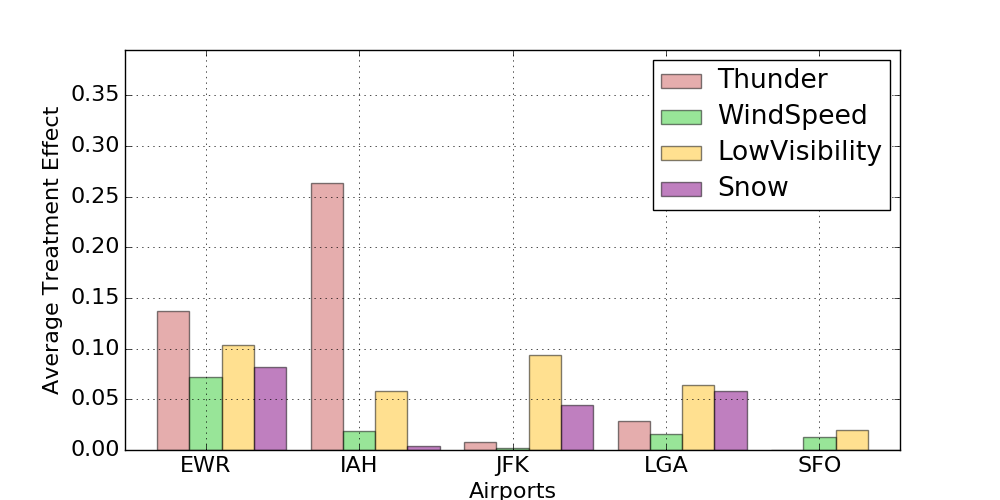
\includegraphics[height=4.3cm,width=1.2\linewidth]{Figures/ATT.png}
\caption{\scriptsize Effect of Weather on Flight Delay}
\label{sfig:testaa}
\end{subfigure}\hfill
\begin{subfigure}{0.33\linewidth}
\centering
\hspace*{-.23cm} 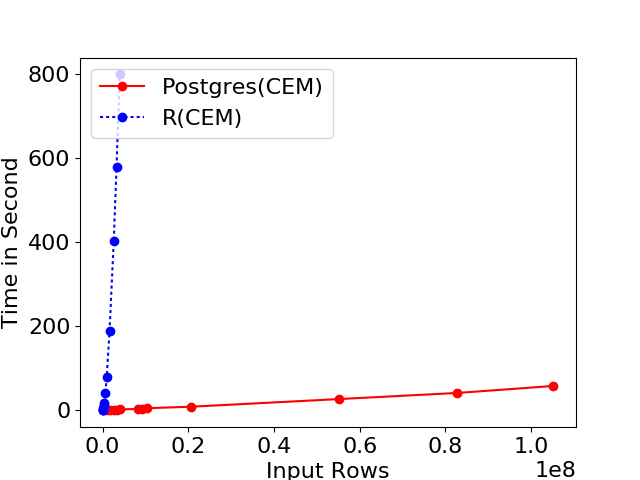
\includegraphics[height=4.3cm,width=1.1\linewidth]{Figures/exact.png}
\caption{\scriptsize Scalability Comparison (Subclassification)}
\label{sfig:testbb}
\end{subfigure}\hfill
\begin{subfigure}{0.33\linewidth}
\centering
\hspace{-.3cm}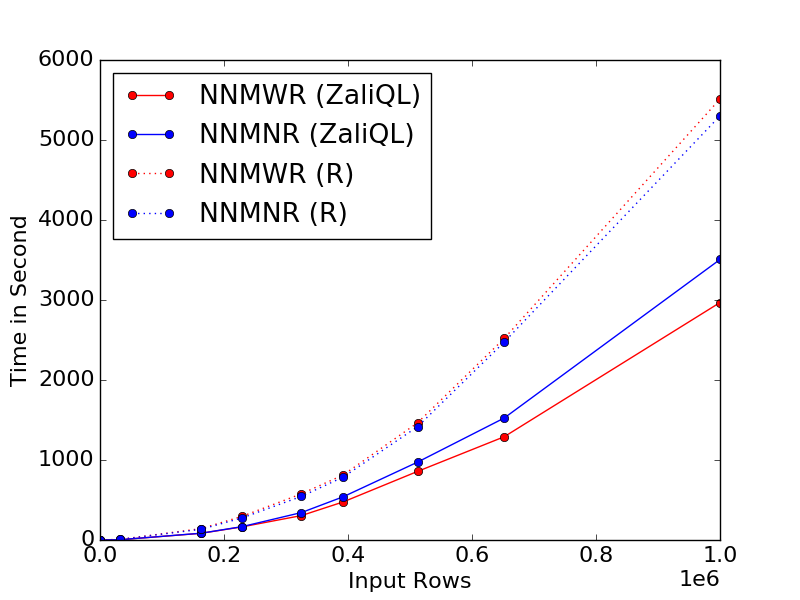
\includegraphics[height=4.3cm,width=1.1\linewidth]{Figures/NNM.png}
\caption{\scriptsize Scalability Comparison (Matching)}
\label{fig:push}
\end{subfigure}\hfill
\caption{{ (Results from preliminary work)~~ Performance and Scalability Evaluation of \GSQL}: we explored: nearest neighbor matching
 with and without replacement (NNMNR and NNMNR, respectively); subclassification bases on exact distance (EM), coarsen exact distance (CEM) and propensity score (Subc.)}
\label{fig:perfresults}
		\vspace{-0.3cm}
\end{figure*}
}

\ignore{
\subsection{Analyzing performance}

 We
explored four candidate causes for flight departure delays and
cancellations: Thunder, WindSpeed, LowVisibility, and Snow.  For
example ``what is the causal effect of {\em Thunder} (a Boolean
attribute in the weather data) on flight departure delay and
cancellation''.  As an illustration, Fig.~\ref{fig:perfresults}(a)
shows the results for delays at various airports: Thunder has the
largest causal effect at IAH (Houston, TX) and EWR
(Newark, NJ), while snow has the largest causal effect at JFK and LGA
(both in New York, NY); we note that these findings are consistent
with the finding. More interestingly we investigated the performance of our
subclassification and matching techniques expressed in SQL with state
of the art tools in R namely, MatchIt \cite{ho1737matchit}
and CEM \cite{iacus2009cem}. The performance for subclassification improves
by two orders of magnitude (Fig.~\ref{fig:perfresults}(b)) and for matching by a
factor of 2 (Fig.~\ref{fig:perfresults}(c)).
}


